\section{\textbf{Background}}
In this section we provide a brief background on the Automata Processor and enumerative techniques for parallelizing FSM processing.
\subsection{NFA and Automata Processor}
A Non-deterministic Finite Automata (NFA) is formally described
by a quintuple $\langle$ Q, $\sum$, $\delta$ , $q_0$ , F$\rangle$, where Q is a set of states,$\sum$  is the
input symbol alphabet, $q_0$ is the set of start states and F is the set 
of reporting or accepting states. The transition function $\delta$(Q,$\alpha$)
defines the set of states reached by Q on input symbol α. The non-determinism is due to the fact that an NFA can have multiple states
active at the same time and have multiple transitions on the same
input symbol.\\
Conventional compute-centric architectures store the complete transition function as a lookup table in the cache/memory. Since a lookup
is required for every active state on every input symbol, symbol processing is bottlenecked by the available memory bandwidth. This
leads to performance degradation especially for large NFAs with
many active states. With limited memory bandwidth, the number
of state transitions that can be processed in parallel is also limited.
Converting these NFAs to equivalent DFAs also cannot help improve
performance since it leads to exponential growth in the number of
states.\\
The memory-centric Automata Processor (AP) accelerates finite
state automata processing by implementing NFA states and state
transitions in memory. Each automata board fits in a DIMM slot
and can be interfaced to a host CPU/FPGA using the DDR/PCIe
interface. Figure 2 illustrates the automata processor architecture.
\begin{figure}[!h]
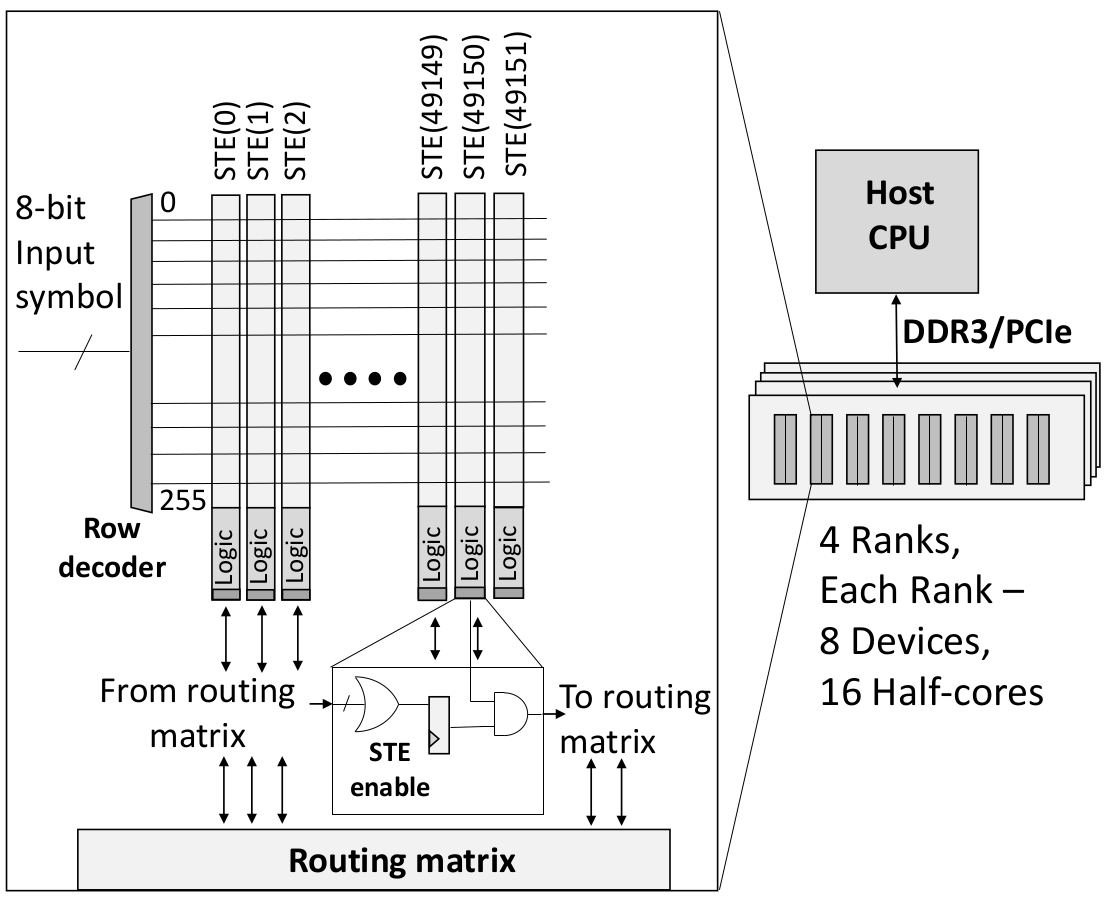
\includegraphics[width=0.50\textwidth]{apoverview.png}
\centering
\caption{An Automata proccesor overview, taken from \cite{1}}
\end{figure}

For processing in AP, the classic representation of NFAs is transformed to a compact ANML NFA representation [12] where each
state has valid incoming transitions for only one input symbol. Thus
each state in an ANML NFA can be labeled by one unique input
symbol. ANML NFA computation entails processing a stream of
input symbols one at a time. Initially, all the start states are active
states. Each step has two phases. In the state match phase, we identify which of the active states have the same label as the current input
symbol. In the state transition phase, we look up the transition table
to determine the destination states for these matched states. These
destination states would become the active states for the next step.
In AP, the FSM states (called State-Transition Elements or STEs)
are stored as columns in DRAM arrays (256 bits). Each STE is
programmed to the one-hot encoding of the 8-bit input symbol (same
as it is label) that it is required to match against. For example, for an
STE to match the input symbol a, the bit position corresponding to
the 97 th row must be set to 1.\\
Each cycle, the input symbol (ASCII alphabet) is broadcast to all
DRAM arrays and serves as the row address. If an STE has a ’1’
bit set in the row, it means that the label of the state it has stored
matches the input symbol. State match is then simply a DRAM row
read operation, with the input symbol as the row address and the
contents of the row determining the STEs that match against the
input symbol. Thus, by broadcasting the input symbol to all DRAM
arrays, it is possible to determine in parallel all the states which
match with the current input symbol.
State transitions between currently active states to next states is
accomplished by a proprietary interconnect (routing matrix) which
encodes the transition function. Reconfiguring this interconnect
requires a costly recompilation step. Only the states which matched
with the current input symbol and are active, undergo state transition.\\
We see how \cite{1} enfasizes how difficult the FMS parallelizing is. Because of the dependencies between every consecutive state transitions.\\
\cite{1} describes the way of parallelization. To parallelize FSM traversal is by partitioning the input string into segments, and processing these segments concurrently. This is feasible because FSM computation can be expressed as a composition of transition functions . Parallelization is possible because transition function composition is associative. Figure 3 shows an example
of parallelizing the FSM with two input segments ($I_1$ and $I_2$ ) each
with five symbols. The FSM shown detects the first word in every
line. The transition table is shown on right. Both these segments can
be executed in parallel to provide a speedup of 2× over sequential
baseline.
However, the starting states for each input segment are unknown
except the first segment (which starts from initial start states). The
starting states for a segment are essentially the ending states of the previous segment. These dependencies prevent concurrent execution
among threads.This problem can be solved by leveraging classic
parallel prefix-sum. The basic idea is to execute the second
segment for every state of the FSM. This method is referred to
as an enumerative computation as it enumerates all possible start
states \cite{2}.
In Figure 3 the start state of the first segment is known ($S_0$)
which is the start state of the FSM. However, the start states of input
segment $I_2$ are unknown. Figure 3 shows an example enumeration
for the second input segment, $I_2$ . This example FSM has 3 states,
so each segment (except the first) enumerates all 3 states. Once the
first segment has finished, it can pick the correct or true paths from
the enumerated paths of the second segment and discard false paths.
Thus, final results can be obtained by combining the intermediate
results of all input segments. The true path for $I_2$ in Figure 3 starts
at $S_1$ , the remaining two paths are false paths. The final path of the
FSM is highlighted.
\begin{figure}[!h]
    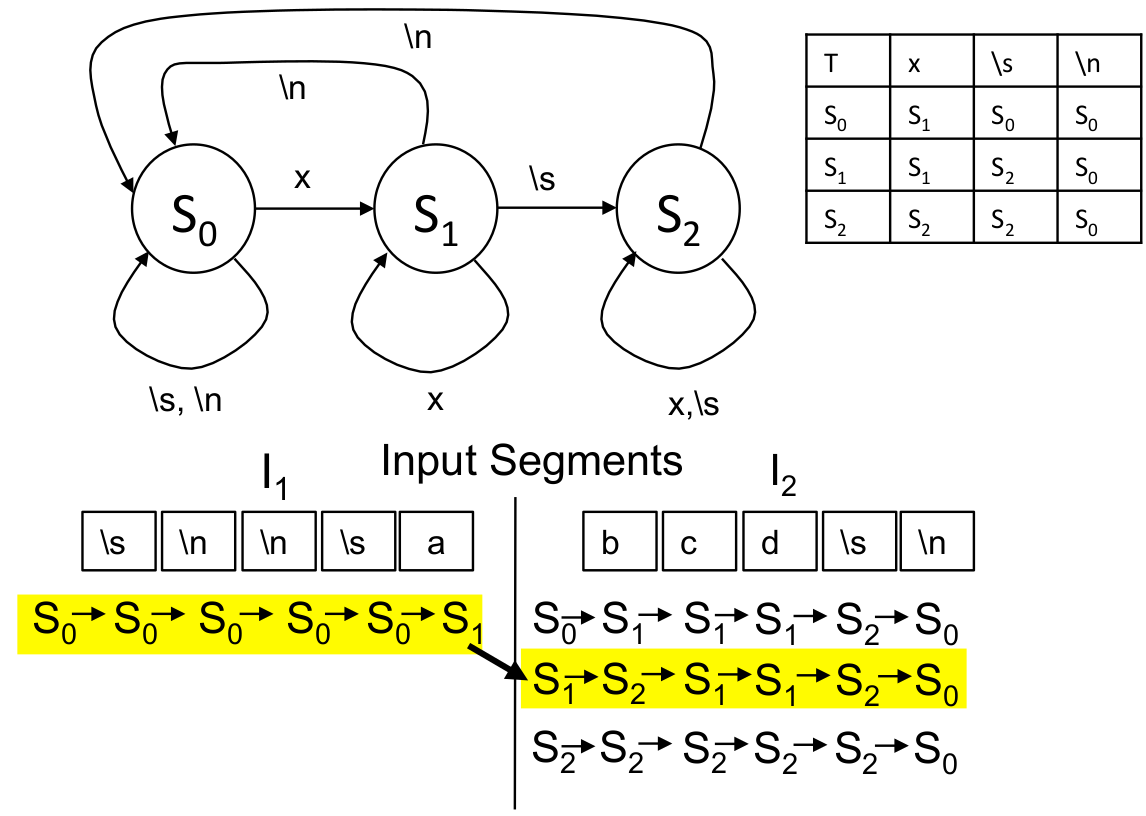
\includegraphics[width=0.50\textwidth]{f3.png}
    \caption{An FSM example with enumeration, taken from \cite{1}}
\end{figure}